\documentclass{beamer}

\usepackage[utf8]{inputenc}
\usepackage{amsmath}

\title{Motion Planning and Control in FTC}
\author{Kelly Muir\\Captain, Team 8367 ACME Robotics}
\date{FIRST Championship Conference Houston 2019}
\logo{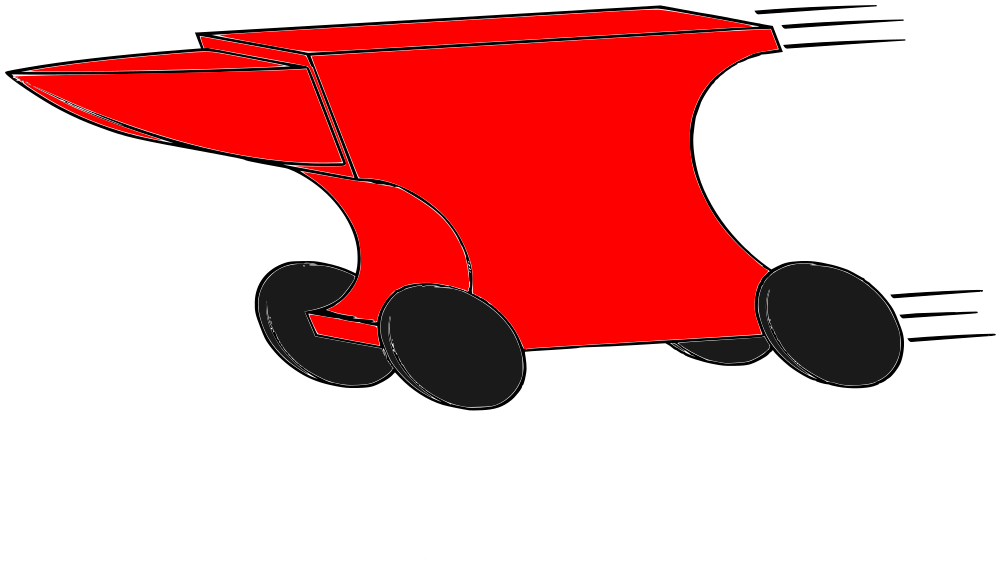
\includegraphics[width=2cm]{./anvil.png}}

\usepackage{listings}
\usepackage{color}

\definecolor{dkgreen}{rgb}{0,0.6,0}
\definecolor{gray}{rgb}{0.5,0.5,0.5}
\definecolor{mauve}{rgb}{0.58,0,0.82}

\lstset{frame=tb,
  language=Java,
  aboveskip=3mm,
  belowskip=3mm,
  showstringspaces=false,
  columns=flexible,
  basicstyle={\small\ttfamily},
  numbers=none,
  numberstyle=\tiny\color{gray},
  keywordstyle=\color{blue},
  commentstyle=\color{dkgreen},
  stringstyle=\color{mauve},
  breaklines=true,
  breakatwhitespace=true,
  tabsize=4
}

\begin{document}

\frame{\titlepage}

\begin{frame}
\frametitle{Terminology}
	\begin{itemize}
		\item {Motion Planning - planning prior to execution of motion}
	\end{itemize}
\end{frame}

\begin{frame}
\frametitle{Terminology}
	\begin{itemize}
		\item {Motion Profile - destribes 1d displacement as a function of time}
	\end{itemize}
\end{frame}

\begin{frame}
\frametitle{Terminology}
	\begin{itemize}
		\item {Path - describes a series of positions for a robot as a function of displacement}
	\end{itemize}
\end{frame}

\begin{frame}
\frametitle{Terminology}
	\begin{itemize}
		\item {Trajectory - Path + Profile, robot state as a function of time}
	\end{itemize}
\end{frame}

\begin{frame}
\frametitle{Terminology}
	\begin{itemize}
		\item {Motion Control - achieving a desired state in a particular system}
	\end{itemize}
\end{frame}

\begin{frame}
\frametitle{Terminology}
	\begin{itemize}
		\item {Feed forward control - predictive control based on known system dynamics}
	\end{itemize}
\end{frame}

\begin{frame}
\frametitle{Terminology}
	\begin{itemize}
		\item {Feed back control - corrective contnrol in reaction to error}
	\end{itemize}
\end{frame}

\begin{frame}
	\frametitle{1D Motion Planning}
	\begin{itemize}
		\item Current State $\rightarrow$ ??? $\rightarrow$ Target State
		\item Constrains: 
			\begin{itemize}
				\item Time optimal
				\item Continuity
				\item Observe physical limitations
			\end{itemize}
	\end{itemize}
\end{frame}

\begin{frame}
	\frametitle{Motion Profiling}
	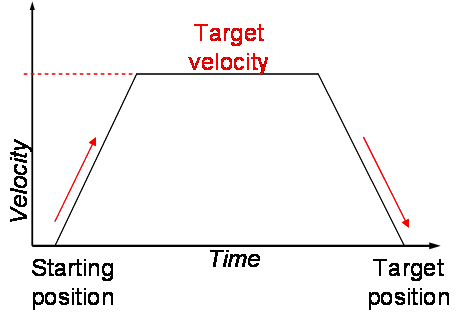
\includegraphics[width=.9\textwidth]{trap.png}
\end{frame}

\begin{frame}
	\frametitle{Motion Profiling}
	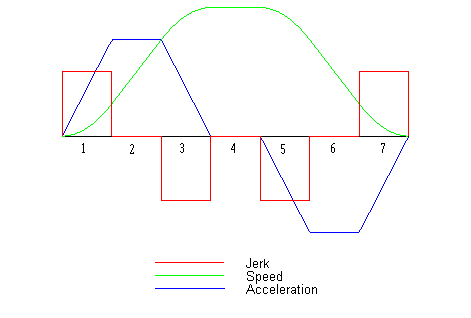
\includegraphics[width=.9\textwidth]{mp.png}
\end{frame}

\begin{frame}
	\frametitle{Motion Profiling}
	\texttt{
MotionProfileGenerator.generateSimpleMotionProfile(
	new MotionState(currentPositon, 0, 0, 0),\\
        new MotionState(targetPosition, 0, 0, 0),\\
        MAX\_V,\\
        MAX\_A,\\
        MAX\_J\\
);
}

\end{frame}
	
\begin{frame}
	\frametitle{Feedforward Control}
	$$voltage  \approx k_\omega \omega + k_\tau \tau$$

	$$v \propto \omega,\; a \propto \tau$$
	
	$$ff(t) = k_v v(t) + k_a a(t) + {some\; friction\; stuff}$$ 

\end{frame}

\begin{frame}
	\frametitle{Tuning}
	\centering
	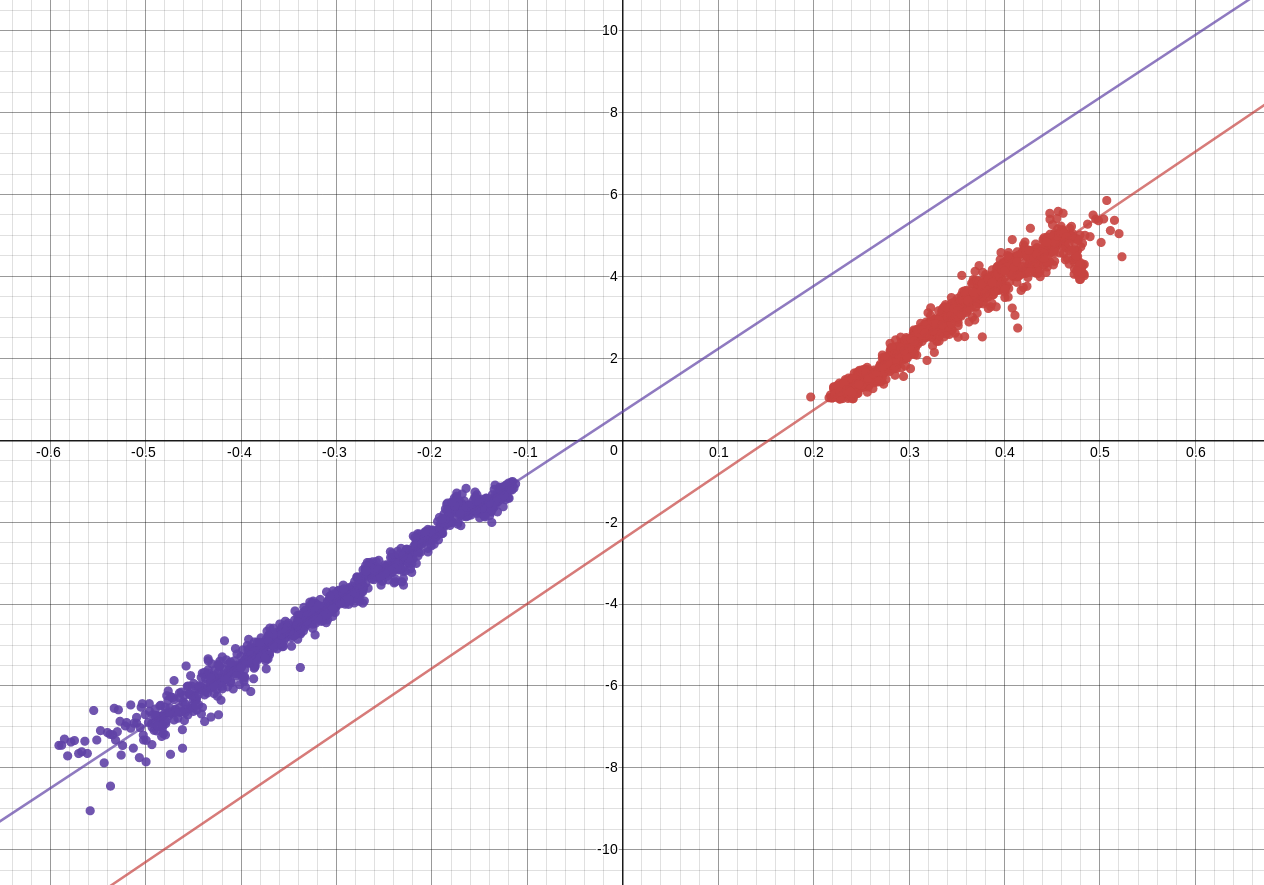
\includegraphics[width=.8\textwidth]{lift1.png}
\end{frame}

\begin{frame}
	\frametitle{PID Control}
	$$c(t) = k_p e(t) + k_i \int_0^t{e(\tau)}d\tau + k_d \frac{d}{dt}e(t)$$ 
	
	\vspace{1cm}

	\textbf{Proportional term:} 
	respond to current error\\
	\textbf{Integral term:} 
	respond to constant state error\\
	\textbf{Derivative term:} 
	respond to change in error\\
\end{frame}

\begin{frame}
	\frametitle{PID Control}
	\begin{centering} 
	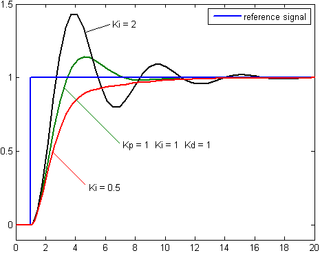
\includegraphics[width=.45\textwidth]{i.png} 
	\hfill
	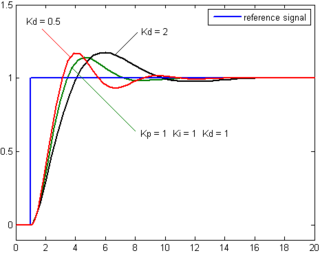
\includegraphics[width=.45\textwidth]{d.png}
	\end{centering}
\end{frame}

\begin{frame}
	\frametitle{PIDF Controller}
	\texttt{
        new PIDFController(\\
	new PIDCoefficients(K\_P, K\_I, K\_D),\\
	K\_V, K\_A, K\_STATIC, (x) -> G);
	}
	\\
	\vspace{1cm}
	\texttt{
		controller.setTargetPosition(target);
	}\\
	\texttt{
		controller.update(currentPosition, targetV, targetA);
		}

\end{frame}



\begin{frame}
	\frametitle{Hermite Splines}
	\centering
	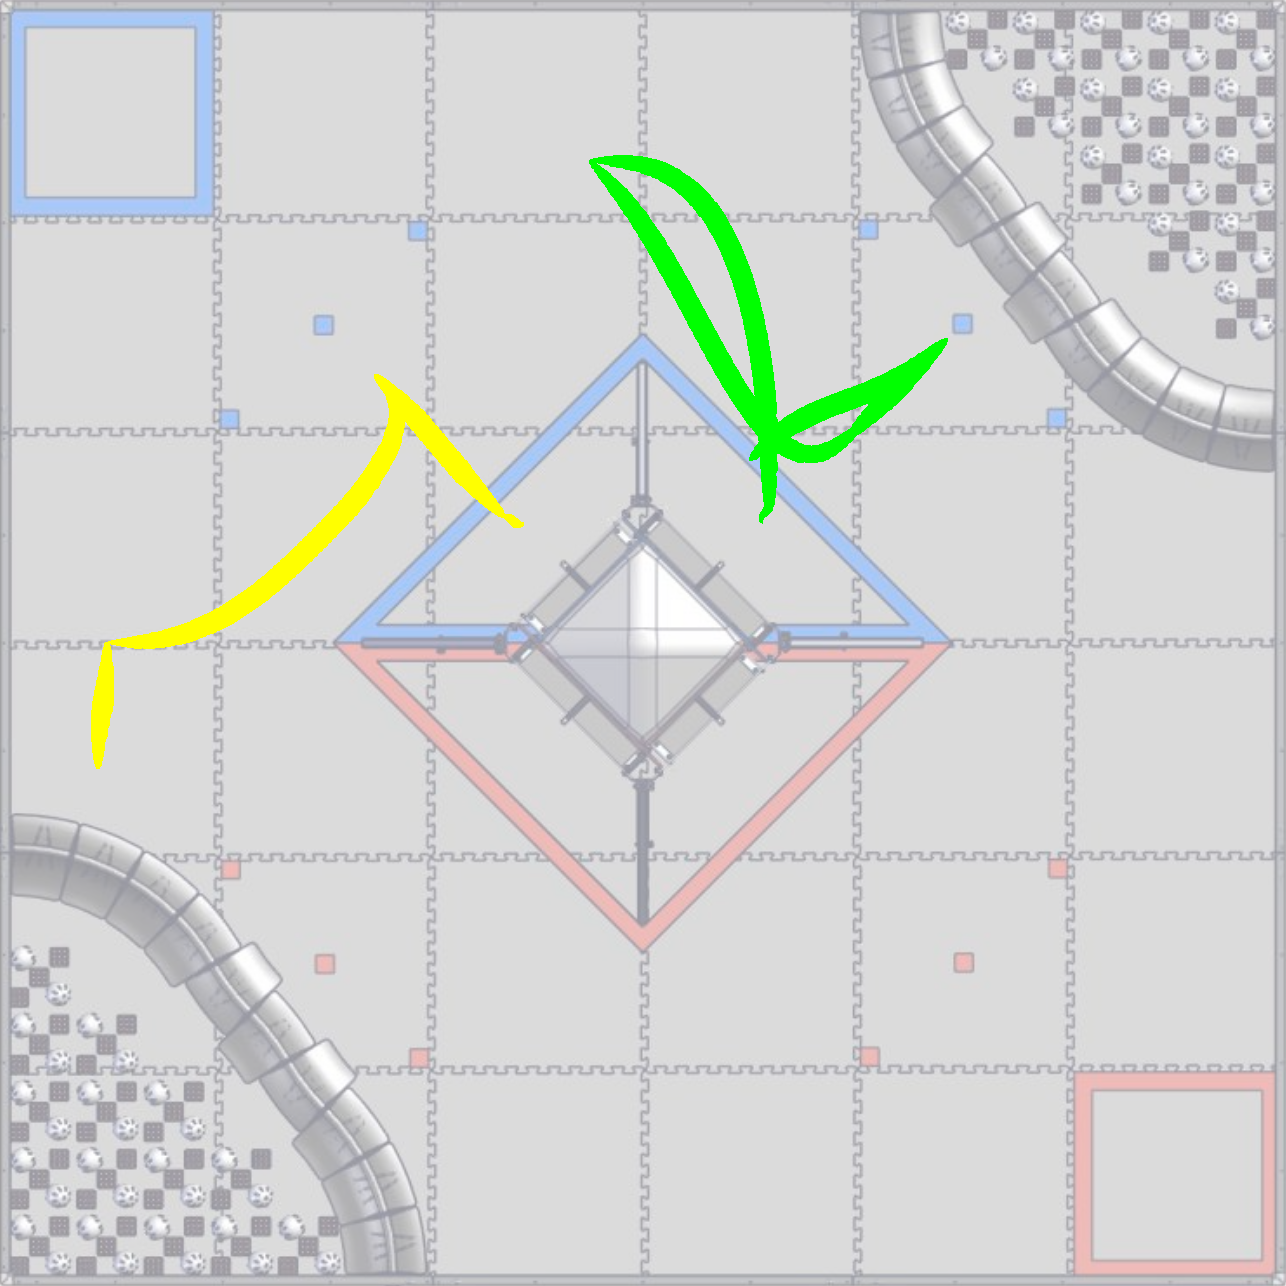
\includegraphics[width=.6\textwidth]{path.png}

\end{frame}

\begin{frame}
	\frametitle{Hermite Splines}
	\centering
	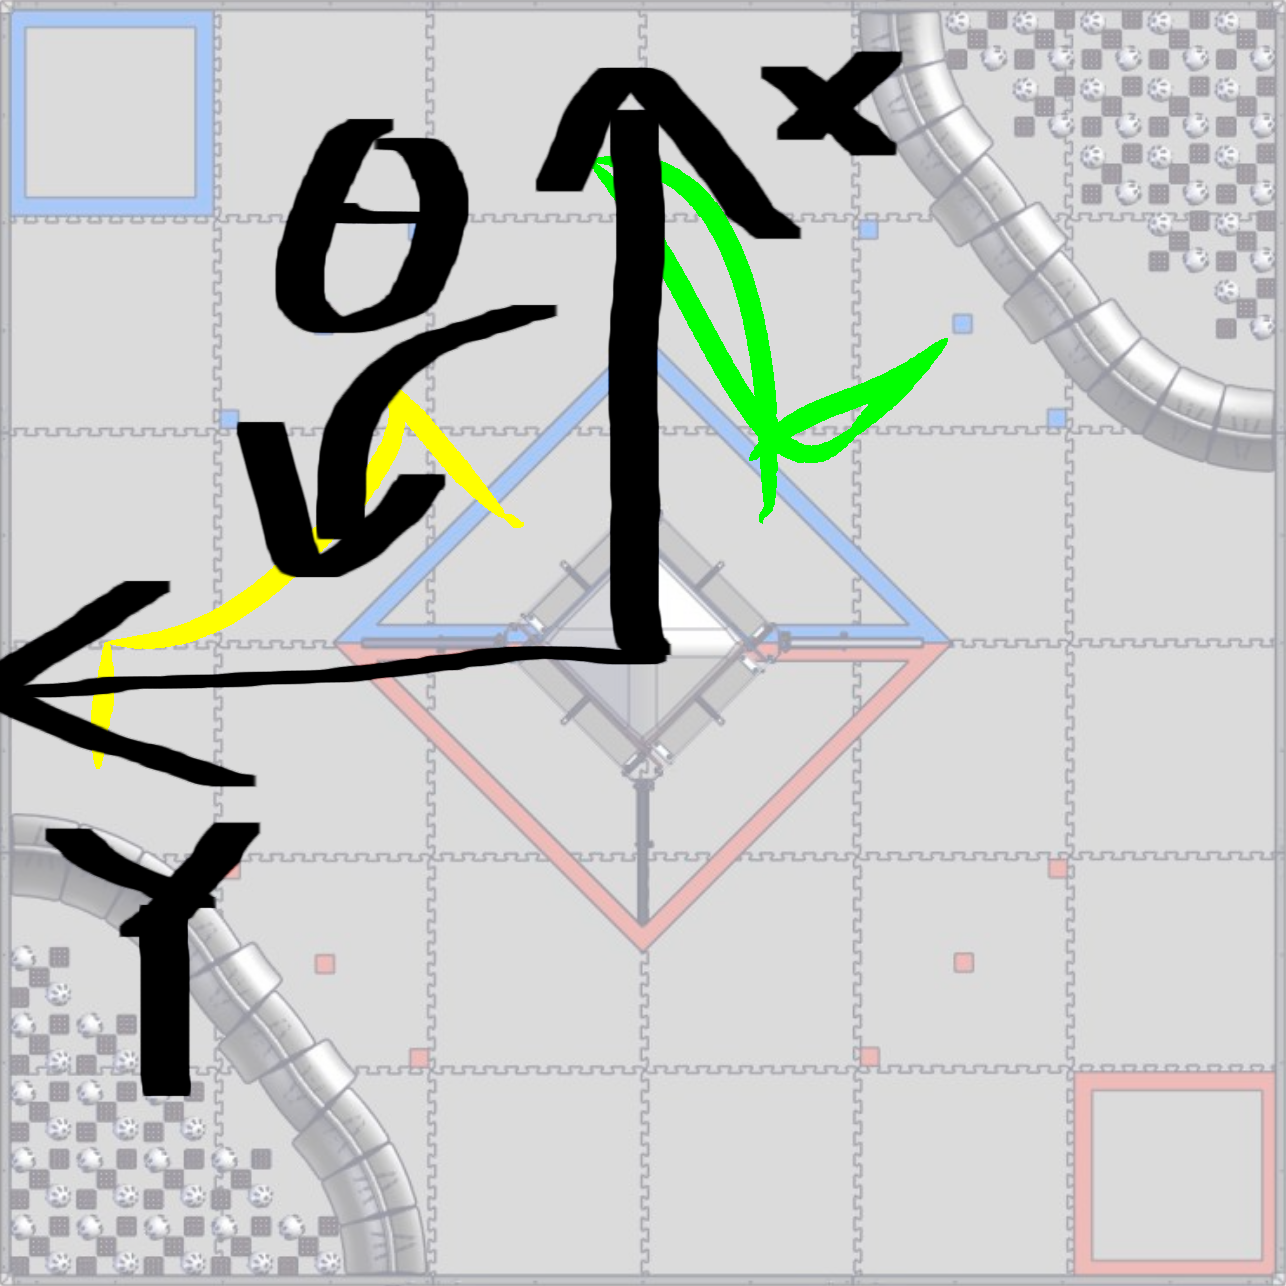
\includegraphics[width=.6\textwidth]{coordinate.png}

\end{frame}

\begin{frame}
	\frametitle{Hermite Splines}
	$$(x, y) = \left( p_x(u), p_y(u) \right)$$

	$$p(u) = au^5 + bu^4 + cu^3 + du^2 + eu + f$$

	\centering
	
	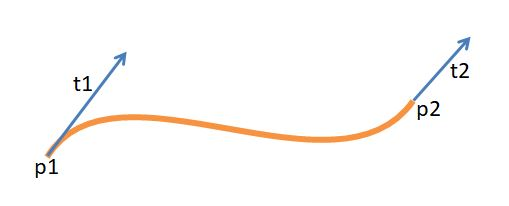
\includegraphics[width=.7\textwidth]{hermite.jpg}

	
\end{frame}

\begin{frame}
	\frametitle{Hermite Splines}
	$$p_x(0) = x_0$$ $$  p_x(1) = x_1$$
	$$p_x'(0) = cos(\theta_0)$$ $$ p_x'(1) = cos(\theta_1)$$
	$$p_x''(0) = 0$$ $$ p_x''(1) = 0$$
	$$p(u) = au^5 + bu^4 + cu^3 + du^2 + eu + f$$
\end{frame}

\end{document}

